\chapter{Complex Langevin dynamics of spherical dimers}
\label{chapter:langevin_dynamics}
Much of the calibration theory discussed in Chapter 2 assumes that the
target particle in question is a single sphere, one who's scattering and 
motion is easily computed. However, while working with dense colloidal 
suspensions, one often ends up trapping more than one sphere. Li and 
Arlt \cite{Li2008} studied the case of two microspheres trapped in a single 
OT and found that multiple trapped beads could be mistaken for a single 
trapped bead with altered trap stiffness. Theoretical studies on the case 
of two trapped microspheres by Xu~\textit{et~al.} \cite{Xu2005} employed a 
ray-optics based model to show that the two trapped beads are brought into 
physical contact with each other by optical forces and they also calculated 
the axial equilibrium positions of the two trapped beads as a function of 
their size. Experiments in \cite{Praveen2016} confirmed that the two trapped 
beads indeed experience different trap stiffnesses in the vicinity of the 
same potential well. There are further discussions looking into the dynamics 
of a whole host of asymmetrically shaped particles \cite{Loudet2014, ShengHua2005, 
Chetana2022}, their results all showing that predicting the behaviour an 
arbitrary shaped particle comes with great difficulty due to the fact that 
the optical force is dependent on a greater number of variables such as 
orientation and size factors.

With the initial goal of the PhD being to induce nucleation events via a 
spherical micro-rotor the goal of this chapter was to - in a limited capacity
simulate and investigate the influence of a second particle being bound to our 
target sphere. The choice of a dimer, instead of an amorphous solid that 
might better represent a growing crystalline solid, allows us to consider 
how the dynamics of the aggregate change by varying the size factor. We build 
upon the works of Vigilante \textit{et al} \cite{Vigilante2020} to consider 
asymmetric dimers and how varying size parameters alters the dynamics and 
additionally makes characterising their interactions within an optical trap 
more cumbersome. Attempting to simulate an amorphous aggregate is rather
difficult as calculating the optical force and torque is computationally 
slow and orientation specific. 

%%%%%%%%%%%%%%%%%%%%%%%%%%%%%%%%%%%%%%%%%%%%%%%%%%%%%%%%%%%%%%%%%%%%%%%%%%%%%%%%
%%%%%%%%%%%%%%%%%%%%%%%%%%%%%%%%%%%%%%%%%%%%%%%%%%%%%%%%%%%%%%%%%%%%%%%%%%%%%%%%
\section{Positional and Orientational dependence of Trapping forces}
\label{sec:eq_positions}
If we wanted to start from first principles and determine the trap strength 
on our target particle the first step would be to locate the equilibrium position
relative to the trap focus. For a single sphere it is easy to enough to understand 
that its centre of mass will be drawn to focal point of the laser due to gradient
forces, once there the force is analogous to a harmonic spring with a fixed trap
stiffness. Now, if we consider instead a dimer, we now have two spheres both being
drawn to the focus along by the same gradient force; in addition the scattering force
is significantly more complex due to both spheres scattering the electromagnetic 
fields. This mutual scattering between individual spheres is what makes simulating
spherical aggregates far more difficult compared to a single sphere, and even harder
still to predict the position where the dimer's centre of mass is in equilibrium.

Because the scattering force is only significant in the direction of beam 
propagation the potential well in the transverse plane can still be assumed 
to be harmonic around the central beam axis. The axial optical force cannot 
be assumed to behave as a simple harmonic trap. The methodology for computing 
optical forces has been covered extensively for a number of different trapping conditions \cite{RanhaNeves2019}, so it is relatively easy to compute the 
trapping force and determine where a simple sphere would be located relative 
to focal point of the laser by finding the position that minimises the net 
optical force in a negative feed back loop ($\delta F/\delta x < 0$) - we can 
assume that for a dielectric sphere the optical torque is negligible. For a 
dimer (or any arbitrary spherical aggregate), we now must consider both its 
position and orientation and find where the net optical force and torque are 
minimised. 

\paragraph{Simulation Parameters}
As a paradigmatic example, consider a dimer suspended in water ($n_p = 1.59, 
n_m = 1.33$) located at the focus of a Gaussian beam (more specifically a Laguerre-Gaussian beam of mode $[0,0]$), the beam is focused by a objective 
with numerical aperture of 1.2 and is x polarised. The size ratio of the two 
sphere's is given by $a_{I}/a_{II} = 2$ where $a_{I}$ is kept at $1\ \mu m$ 
unless specified otherwise; the dimer's orientation is given by a unit vector connecting the centres of both spheres, we define the 'standard' orientation 
as being aligned with the direction of beam propagation direction - and 
therefore the 'inverted' orientation is defined when the dimer is orientated 
against the direction of beam orientation (see figures~\ref{fig:paradigmatic}(b) 
and (d)). 

After computing its $T$-matrix via \textit{mstm} and supplying that 
to \textit{ott} we compute the optical force via \eqref{eq:optical_force} 
in the axial direction while the dimer is in its 'standard' orientation. 
As expected we see a single point where the dimer will be in equilibrium, 
the linear fit in fig.~\ref{fig:paradigmatic}(a) indicates a that the force 
can be modelled as a harmonic potential close to the equilibrium position ($F_z\approx-\kappa_z z$). The second point where the axial 
force goes to 0 cannot be considered as equilibrium position as the positive 
gradient indicates that the trap is unstable unless Brownian motion is ignored. 

We repeated the same calculation but now while the dimer is in its 'inverted' orientation, instead of a single point where the optical force is minimised we 
see that there are instead two separate equilibrium positions, one above the focus
and one below the focus. In this particular example the two positions are far enough
apart that both can be considered as separate harmonic traps.    
\begin{figure}[h!]
	\centering
	\begin{subfigure}{.75\linewidth}
		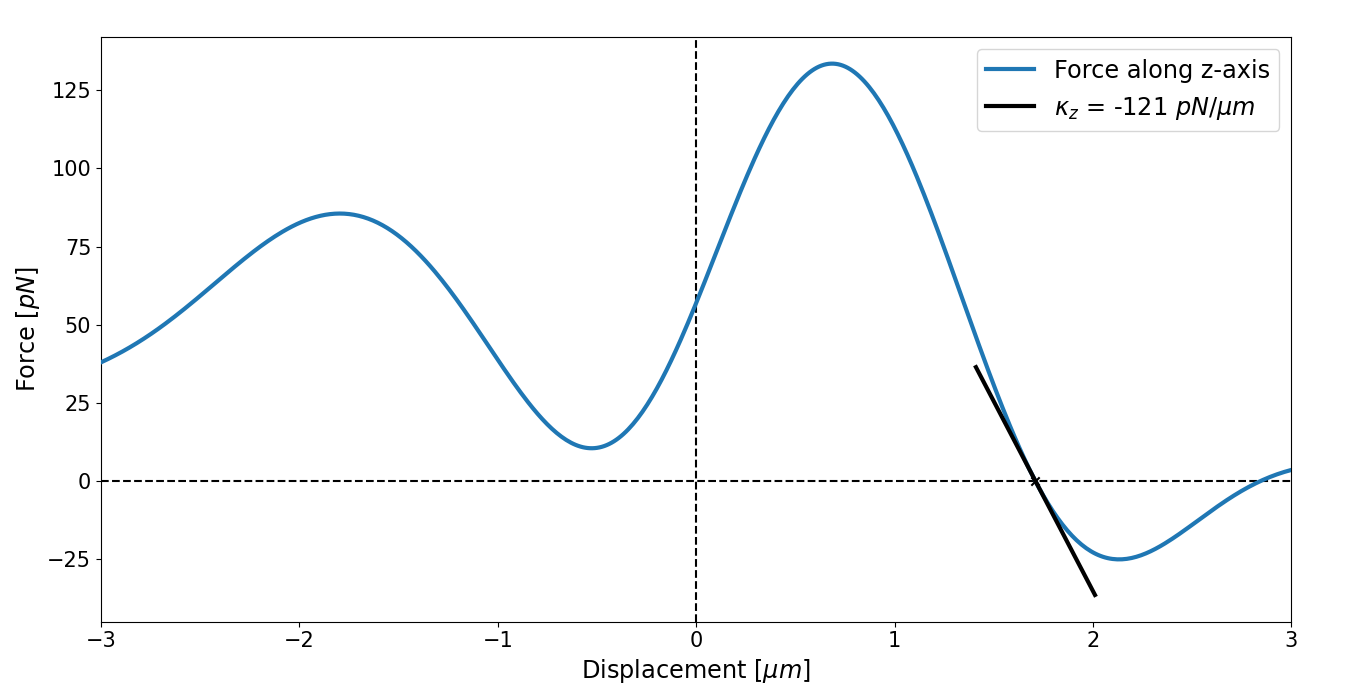
\includegraphics[width=\linewidth]{lam=2_theta=0.png}
		\caption{}
		\label{lam=2}
	\end{subfigure}\hfill % <-- "\hfill"
	\begin{subfigure}{.25\linewidth}
		\centering
		\raisebox{50pt}[0pt][0pt]{\makebox{}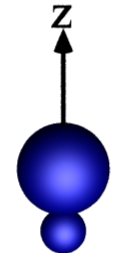
\includegraphics[width=0.3\linewidth, keepaspectratio]{theta=0.png}}
		\caption{}
		\label{large over small}
	\end{subfigure}
	\medskip
	\begin{subfigure}{.75\linewidth}
		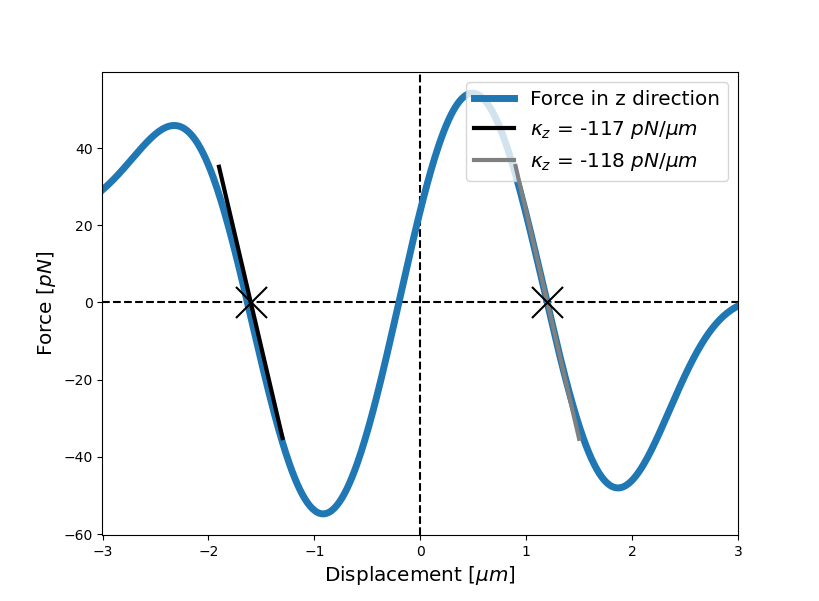
\includegraphics[width=\linewidth]{lam=2_theta=180.png}
		\caption{}
		\label{lam=2_inverted}
	\end{subfigure}\hfill % <-- "\hfill"
	\begin{subfigure}{.25\linewidth}
		\centering
		\raisebox{30pt}[0pt][0pt]{\makebox{}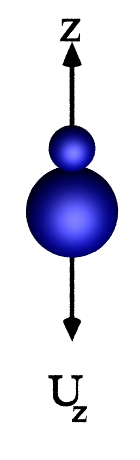
\includegraphics[width=0.3\linewidth, keepaspectratio]{theta=180.png}}
		\caption{}
		\label{small_over_large}
	\end{subfigure}
	\caption{Plots of force vs displacement of the centre of mass of 
		the dimer (µm) for the case of a dimer of size ratio 2. (a) is 
		the case where the dimer is in its' 'standard' orientation. 
		(c) is the case where the dimer is in its' 'inverted' orientation 
		(b) and (d) are renders to visualise the dimer orientation are shown 
		below each plot. The black lines on each force-curve is a linear 
		fit with the slope being reported as the trap stiffness in the legend.}
		\label{fig:paradigmatic}
\end{figure}

We can see that both equilibrium positions have comparable axial trap stiffness 
($\kappa_z$), however the difference in the transverse trap stiffness ($\kappa_x$) 
is far more noticeable. As shown in Fig~\ref{fig:transverse_force}, 
the dimer's orientation and relative position significantly changes the force 
curve; not only is the trap wider when inverted but the trap stiffness is 
increased. This highlights one of the challenges involved with studying 
asymmetric particles, even though its a simple enough process to trap them 
they maybe characterised very differently depending on their relative position 
and orientation towards the focus. This can have a significant impact on 
rheological studies - or attempting to probe any local property - as the 
variance in trap strength can result in large errors over repeated measurements. 
\begin{figure}[h!]
	\centering
	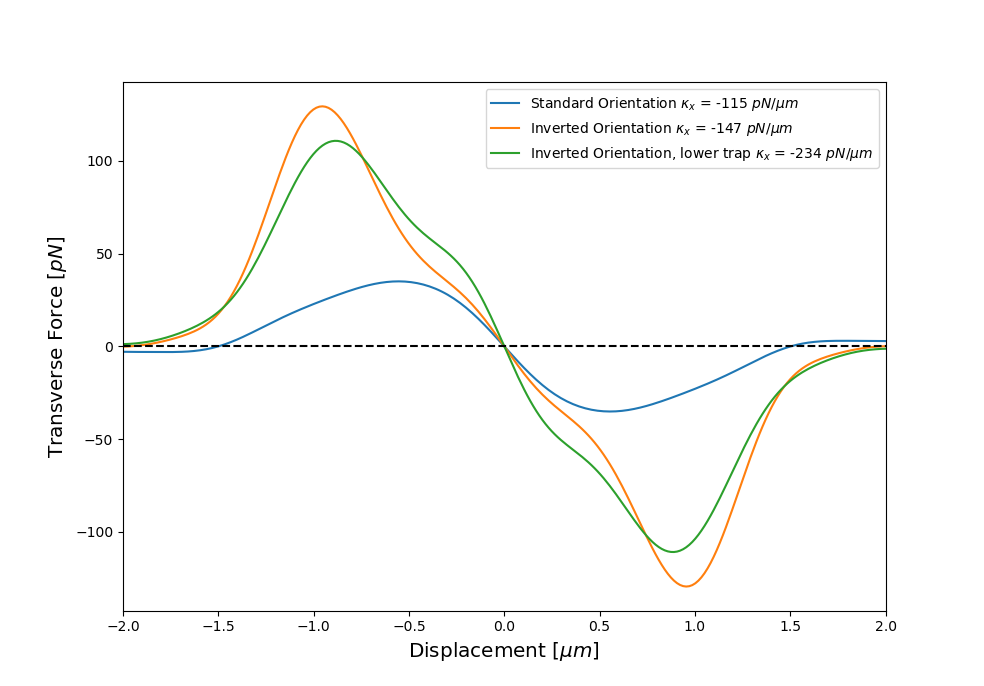
\includegraphics[width=\linewidth]{transverse_force.png}
	\caption{Plots of force vs displacement of the dimer's centre of mass spheres, 
		where a positive force indicates the dimer is directed right on the x-axis, 
		and vice versa for a negative force. The same simulation parameters are used here as in fig~\ref{fig:paradigmatic}(a) and (c). The blue curve representing the force response for a dimer in its standard orientation, orange being the inverted case, and green the same case but placed below the focus.}
	\label{fig:transverse_force}
\end{figure}

For completeness the harmonic traps were located for dimers across a range 
of size ratios - from $a_{I}/a_{II} = 1$ to $a_{I}/a_{II}=10$ - while also 
recording the trap stiffness for each trap. The same simulation parameters are 
used here as for figures \ref{fig:paradigmatic} \& \ref{fig:transverse_force}. 
As shown in Fig.~\ref{fig:eq_positions} $a_{II}$ decrease the dimer begins to
approximate a single homogenous sphere - at least in terms of location and trap strength. However, for intermediate sized dimers (between $a_{I}/a_{II} = 1.1$ 
to $a_{I}/a_{II}=4$), a second equilibrium position is found below the trapping 
focus. Previous work using the ray-optics model have confirmed even in the case 
that two spheres begin separated the electric field will align the particles as 
such that they make contact and are trapped together about a single trapping 
position \cite{Xu2005}. Furthermore it has been shown through proper manipulation 
of the Gaussian or Bessel beam modes that any number of trapping potentials can 
be developed \cite{Shahabadi2020} for nanoparticles. This result however, is the 
first example of an orientation dependent trapping situation using only a 
$TEM_00$ beam. Typical experimental arrangements cannot determine much information 
on the axial position of a trapped particle relative to the trap focus; this 
result indicates not only that dimers can be trapped in multiple axial positions 
but also their trapping behaviour is heavily dependent on said axial position. 
As such it is necessary that positional information in the z-axis can be elucidated
if multiple spheres are trapped simultaneously. 

\begin{figure}[h!]
	\centering
	\begin{subfigure}{0.85\linewidth}
		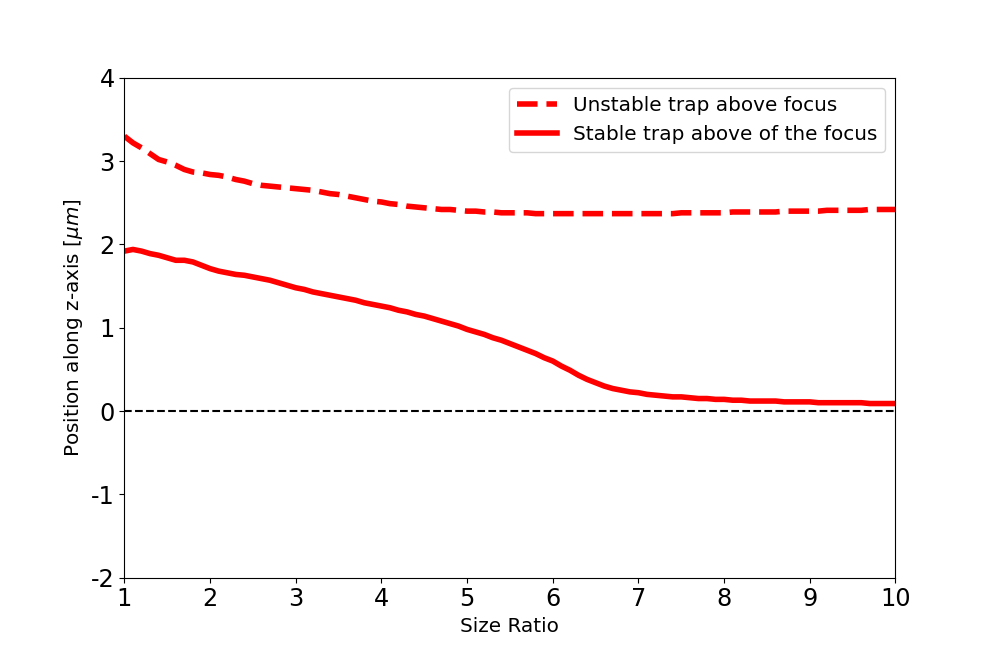
\includegraphics[width=\linewidth]{Equillibrium_positions.png}
		\caption{}
		\label{eq_pos}
	\end{subfigure}\hfill % <-- "\hfill"
	\medskip
	\begin{subfigure}{0.85\linewidth}
		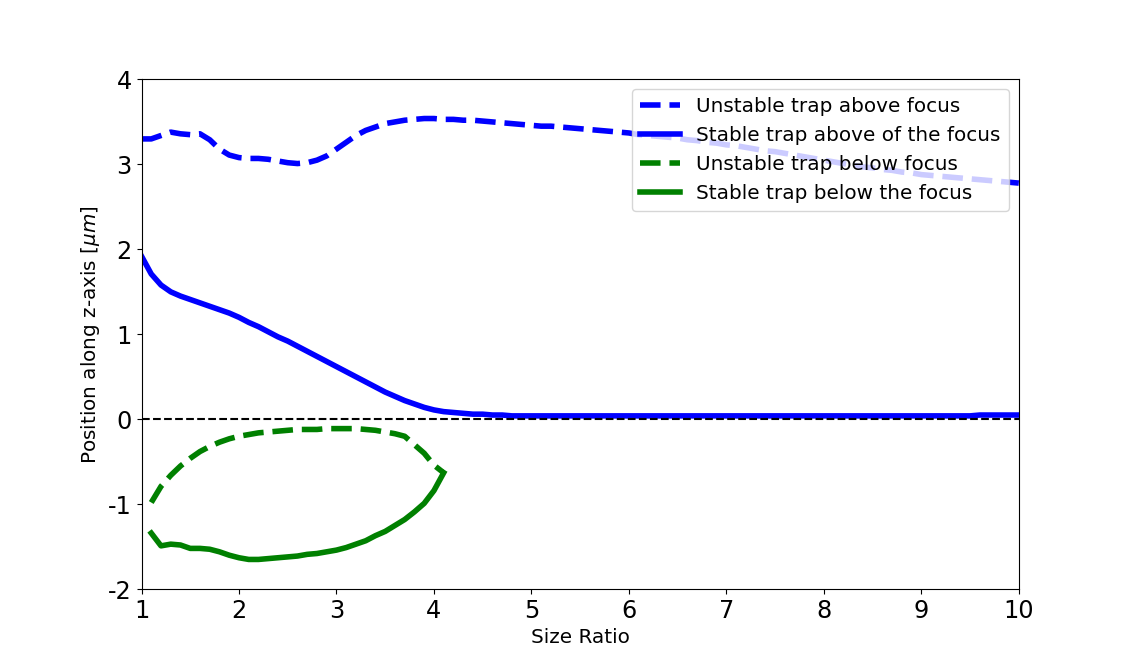
\includegraphics[width=\linewidth]{Equillibrium_positions_inverted.png}
		\caption{}
		\label{eq_pos_inverted}
	\end{subfigure}
	\caption{Equilibrium positions of optically trapped dimers with varying 
		size ratio, dashed lines represent unstable traps whereas solid lines 
		are for stable equilibrium positions. (a) shows that dimers while in their
		'standard' orientation will always have a single equilibrium position. 
		(b) shows that when the same dimer is in its' 'inverted' orientation 
		can be trapped in two axial positions, one below the focus and one above 
		the focus.}
	\label{fig:eq_positions}
\end{figure}

\newpage
\subsection{Non-trivial equilibrium configurations}
\label{sec:off-axis}
Computing the equilibrium positions when a dimer is aligned with the electric 
field is relatively simple as the orientational torque is minimised (see
Eq.\ref{eq:opt_torque}), meaning once trapped the dimer is unlikely to change
orientation enough to escape the trap. However, that does not rule out the 
possibility that there is a stable configuration where the orientation not 
strictly vertical, in fact most experimental work with symmetric nano-dimers 
will trap them lying perpendicular to the beam direction \cite{Ahn2018, 
Reimann2018}. Unlike in Sec.~\ref{sec:eq_positions} we cannot simply measure 
the optical force and torque as the parameter space is too large and determining 
if a particular position and orientation is stable is not clear based solely 
on force and torque measurements \cite{Bui2017}. Using the same simulation 
parameters as before we ran a number short simulations (total simulation time 
was $0.005$ s) with the laser power increased to $500\ mW$. Each simulation 
started with the dimer in a different starting position and orientation, due 
to the high laser power the dimers either escaped the trap or were stably 
trapped. The $z-\theta$ phase space - where $\theta$ is the angle between the 
direction of beam propagation and the dimer's orientation vector ($\theta=0^
\circ$ is the 'standard' orientation) - can be divided into different regions 
depending on which equilibrium configuration is reached.

\begin{figure}[h!]
	\centering
	\begin{subfigure}{0.67\linewidth}
		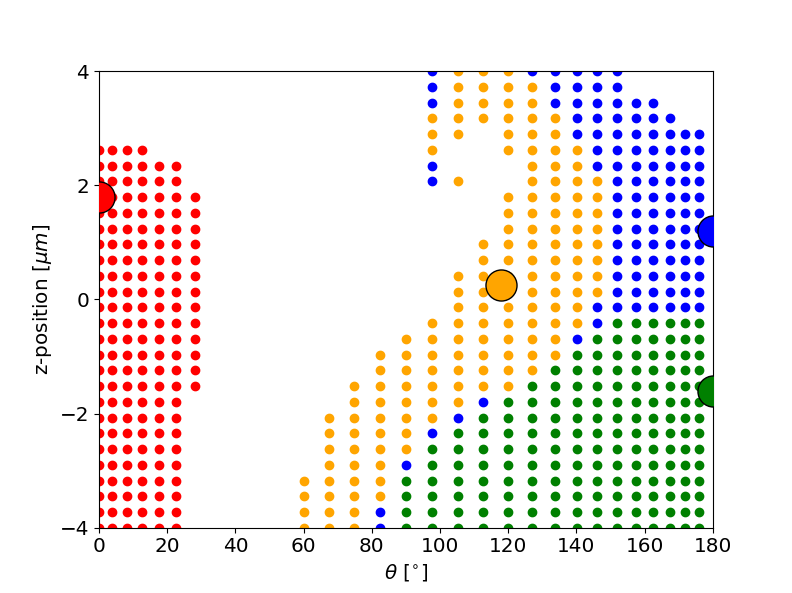
\includegraphics[width=\linewidth]{off_axis_trap.png}
	\end{subfigure}
	\begin{subfigure}{0.32\linewidth}
		\raisebox{0pt}[0pt][0pt]{\makebox{}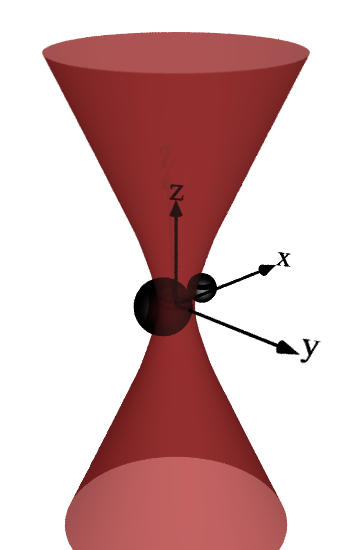
\includegraphics[width=\linewidth, keepaspectratio]{off_axis_render.png}}
		\caption{}
	\end{subfigure}
	%\captionsetup{hangindent=2.35cm}
	\caption{Map of $z-\theta$ phase space using a dimer of size ratio 2 with 
		a laser power of 500 mW ($\theta=0\circ$ is the 'standard' orientation 
		and $\theta=180^\circ$ is the 'inverted' orientation). The stable 
		configurations are indicated by the larger circles and the starting 
		conditions are colour coded to match the stable point they end up in. 
		Right hand render shows a dimer in its off-axis configuration.}
	\label{fig:off_axis}
\end{figure}

Interestingly while the trap strength of these off-axis traps are similar 
in magnitude to the vertically aligned dimers, but when the laser power 
is lowered (around $5\ mW$) the traps become metastable; after reaching its'
equilibrium configuration the particle behaves similarly to a typically
trapped dimer but the trapping potential is small enough that the dimer
escapes in as little time as less than a second or after nearly a full 
3 seconds. Running similar simulations but for vertical configurations 
sees the dimer remaining trapped, even after 30 seconds of run time, 
indicating that the trapping potential is far greater than the thermal 
energy. This suggests that the reason this off-axis configuration is due 
to the rotational motion more than translational motion. If the overall 
potential depth could be characterised then dimers placed into this 
orientation could be used as a micro-scale temperature alarm, where 
by fine tuning of the dimer's parameters would allow you to construct a 
potential well that can only be escaped when the local fluid temperature 
exceeds a certain maximum value.  

%%%%%%%%%%%%%%%%%%%%%%%%%%%%%%%%%%%%%%%%%%%%%%%%%%%%%%%%%%%%%%%%%%%%%%%%%%%%%%%%
%%%%%%%%%%%%%%%%%%%%%%%%%%%%%%%%%%%%%%%%%%%%%%%%%%%%%%%%%%%%%%%%%%%%%%%%%%%%%%%%
\section{Continuous rotational motion due to second-order scattering}

One aspect that has yet to be covered in depth with regards to
spherical aggregates of any construction is their interaction with
circularly polarised light. While most homogenous objects are trapped
no differently in different polarisations, dimers have been shown to
experience an optical torque \cite{Vigilante2020, Ahn2018, Reimann2018}. 
Typically the spin density of an electric field cannot be reduced in 
homogenous medium due to the fact that the spin angular momentum is 
conserved locally. In which case the only way to transfer angular 
momentum to use an object that is anisotropic. This is seen most 
clearly with birefringent materials, due to fact that the crystal 
lattice itself is anisotropic, a circularly polarised beam will 
transfer an optical torque that is proportional to the difference in 
the refractive index of the particle's ordinary and extraordinary axis. 
The total optical torque is given as:
\begin{equation}
	\label{eq:opt_torque}
	\begin{aligned}
		\tau_{opt} =& -\frac{\epsilon}{2\omega_{laser}}E_0^2sin(kd(\Delta n))cos2\theta sin2\phi \\ &+  \frac{\epsilon}{2\omega_{laser}}E_0^2 (1-cos(kd(\Delta n))sin2\phi)
	\end{aligned}
\end{equation}

Where $\Delta n$ is the difference in refractive indices of the 
particle, $\phi$ indicates the phase shift in the electric field
(for circular polarised light $\phi= \pi/4$), and $\theta$ is the angle
between the particle's main axis and the direction of the electric field.
The optical torque of non-birefringent spherical aggregates has no such 
relationship as the mechanism behind their rotation is not as clearly defined. 

To visualise the relationship between the polarisation state of the 
trapping beam, and the rotation rate we simulated the motion of an 
optically trapped dimer in beams of varying polarisation ($NA=1.2$, 
$P=100\ mW$), and the dimer is composed of silica ($n_p=1.59$, 
$n_m=1.33$). Each simulation was run for $1$ second ($\Delta t 
=10^-5$) and at the end we looked at the orientational time series; 
the dimer's orientation is recorded as a quaternion which can be easily 
converted to a 3-dimensional rotation matrix. By considering only the 
transverse components ($U_{1,x}$, $U_{1,y}$, $U_{2,x}$, \& $U_{2,y}$) 
of the rotation matrix and taking the Fourier transformation of their 
time series reveals the rotational frequency. The laser power is set to 
$100\ mW$ to avoid large rotational fluctuations and so that the Fourier 
series of the transverse components approximates $\delta(\omega_{rot}-f)$ 
- the Dirac delta function centred at the rotational frequency $\omega_{rot}$.

%% Example plot of rotating beam trajectory and then the same thing but 
%% Fourier transformed
\begin{equation}
\begin{split}
	q(t) \rightarrow R(t) =& 
	\begin{pmatrix}
		U_{1,x}(t) && U_{2,x}(t) && U_{3,x}(t) \\
		U_{1,y}(t) && U_{2,y}(t) && U_{3,y}(t) \\
		U_{1,z}(t) && U_{2,z}(t) && U_{3,z}(t) 
	\end{pmatrix} \\
	\rightarrow
	&\int^\infty_{-\infty}R(t)e^{-i2\pi ft} dt = 
	\begin{pmatrix}
		\delta(\omega_{rot}-f) && \delta(\omega_{rot}-f) && \delta(f) \\
		\delta(\omega_{rot}-f) && \delta(\omega_{rot}-f) && \delta(f)\\
		\delta(f) && \delta(f) && \delta(f)
	\end{pmatrix}
\end{split}
\end{equation}

If the rotational frequency was not immediately obvious the simulation was
repeated but over a longer simulation time. Four different size ratio of 
dimers were studied, both in their 'standard' and 'inverted' orientations. 
The results of this are displayed in Fig.~\ref{fig:rotation_vs_pol}:
\begin{figure}[h!]
	\centering
	\includegraphics[width=\linewidth]{rotation_vs_pol.png}
	\caption{Rotation frequency vs component phase difference for differently 
		sized dimers. The solid lines represent the rotation rate experienced 
		while the dimer is in its standard orientation, whereas the solid points 
		are for the case where the orientation is inverted. Laser power $= 100\ mW$.}
	\label{fig:rotation_vs_pol}
\end{figure}

A possible explanation of this phenomena was devised by by \cite{Yevick2017}, 
who found that highly focused Gaussian beams could produce second 
order effects in the Rayleigh regime resulting in a photo-kinetic 
force that results in orbital motion about the beam's central axis.
This was verified by \cite{Ruffner2012} who found that by trapping 
a silica bead and recording its position over the course of several 
minutes; while not immediately evident from the trajectory by measuring 
the probability flux of finding a particle in a given position 
revealed a helicity to the sphere's motion which matched the helicity 
of the trapping beam. This would hardly be considered similar to 
the behaviour shown by dimers; firstly because the probability flux 
is an indicator of the sphere's position not its orientation - the 
sphere can be thought to 'orbit' around the central beam axis with a 
radius of orbit on the order of $10^{-9}\ m$. Secondly, while 
\cite{Yevick2017} does compute a rotational frequency, for a single 
sphere this rotation rate is at most $0.01\ Hz$ whereas the lowest 
rotation rate recorded for a dimer ($a_{I}/a_{II}$) was around $2\ Hz$, 
a full two orders of magnitude greater. As such the rotation demonstrated
cannot be explained due to photo-kinetic forces.

This rotation was first noted by Vigilante and co-workers who only 
considered this behaviour for a symmetric dimer \cite{Vigilante2020}; 
to expand upon this work we looked at how the rotation rate changed
with the dimers' size ratio ($a_{I}/a_{II}$) and if the orientation
of the dimer plays any impact on the rotational frequency. By repeating
the same kinds of simulation as used in \ref{fig:rotation_vs_pol} but for
a circularly polarised beam $\phi=90\circ$ it was found that not only is 
the rotation rate dependent on the size of the dimer, but also on its 
orientation and therefore their axial position.
\begin{figure}[h!]
  \centering
  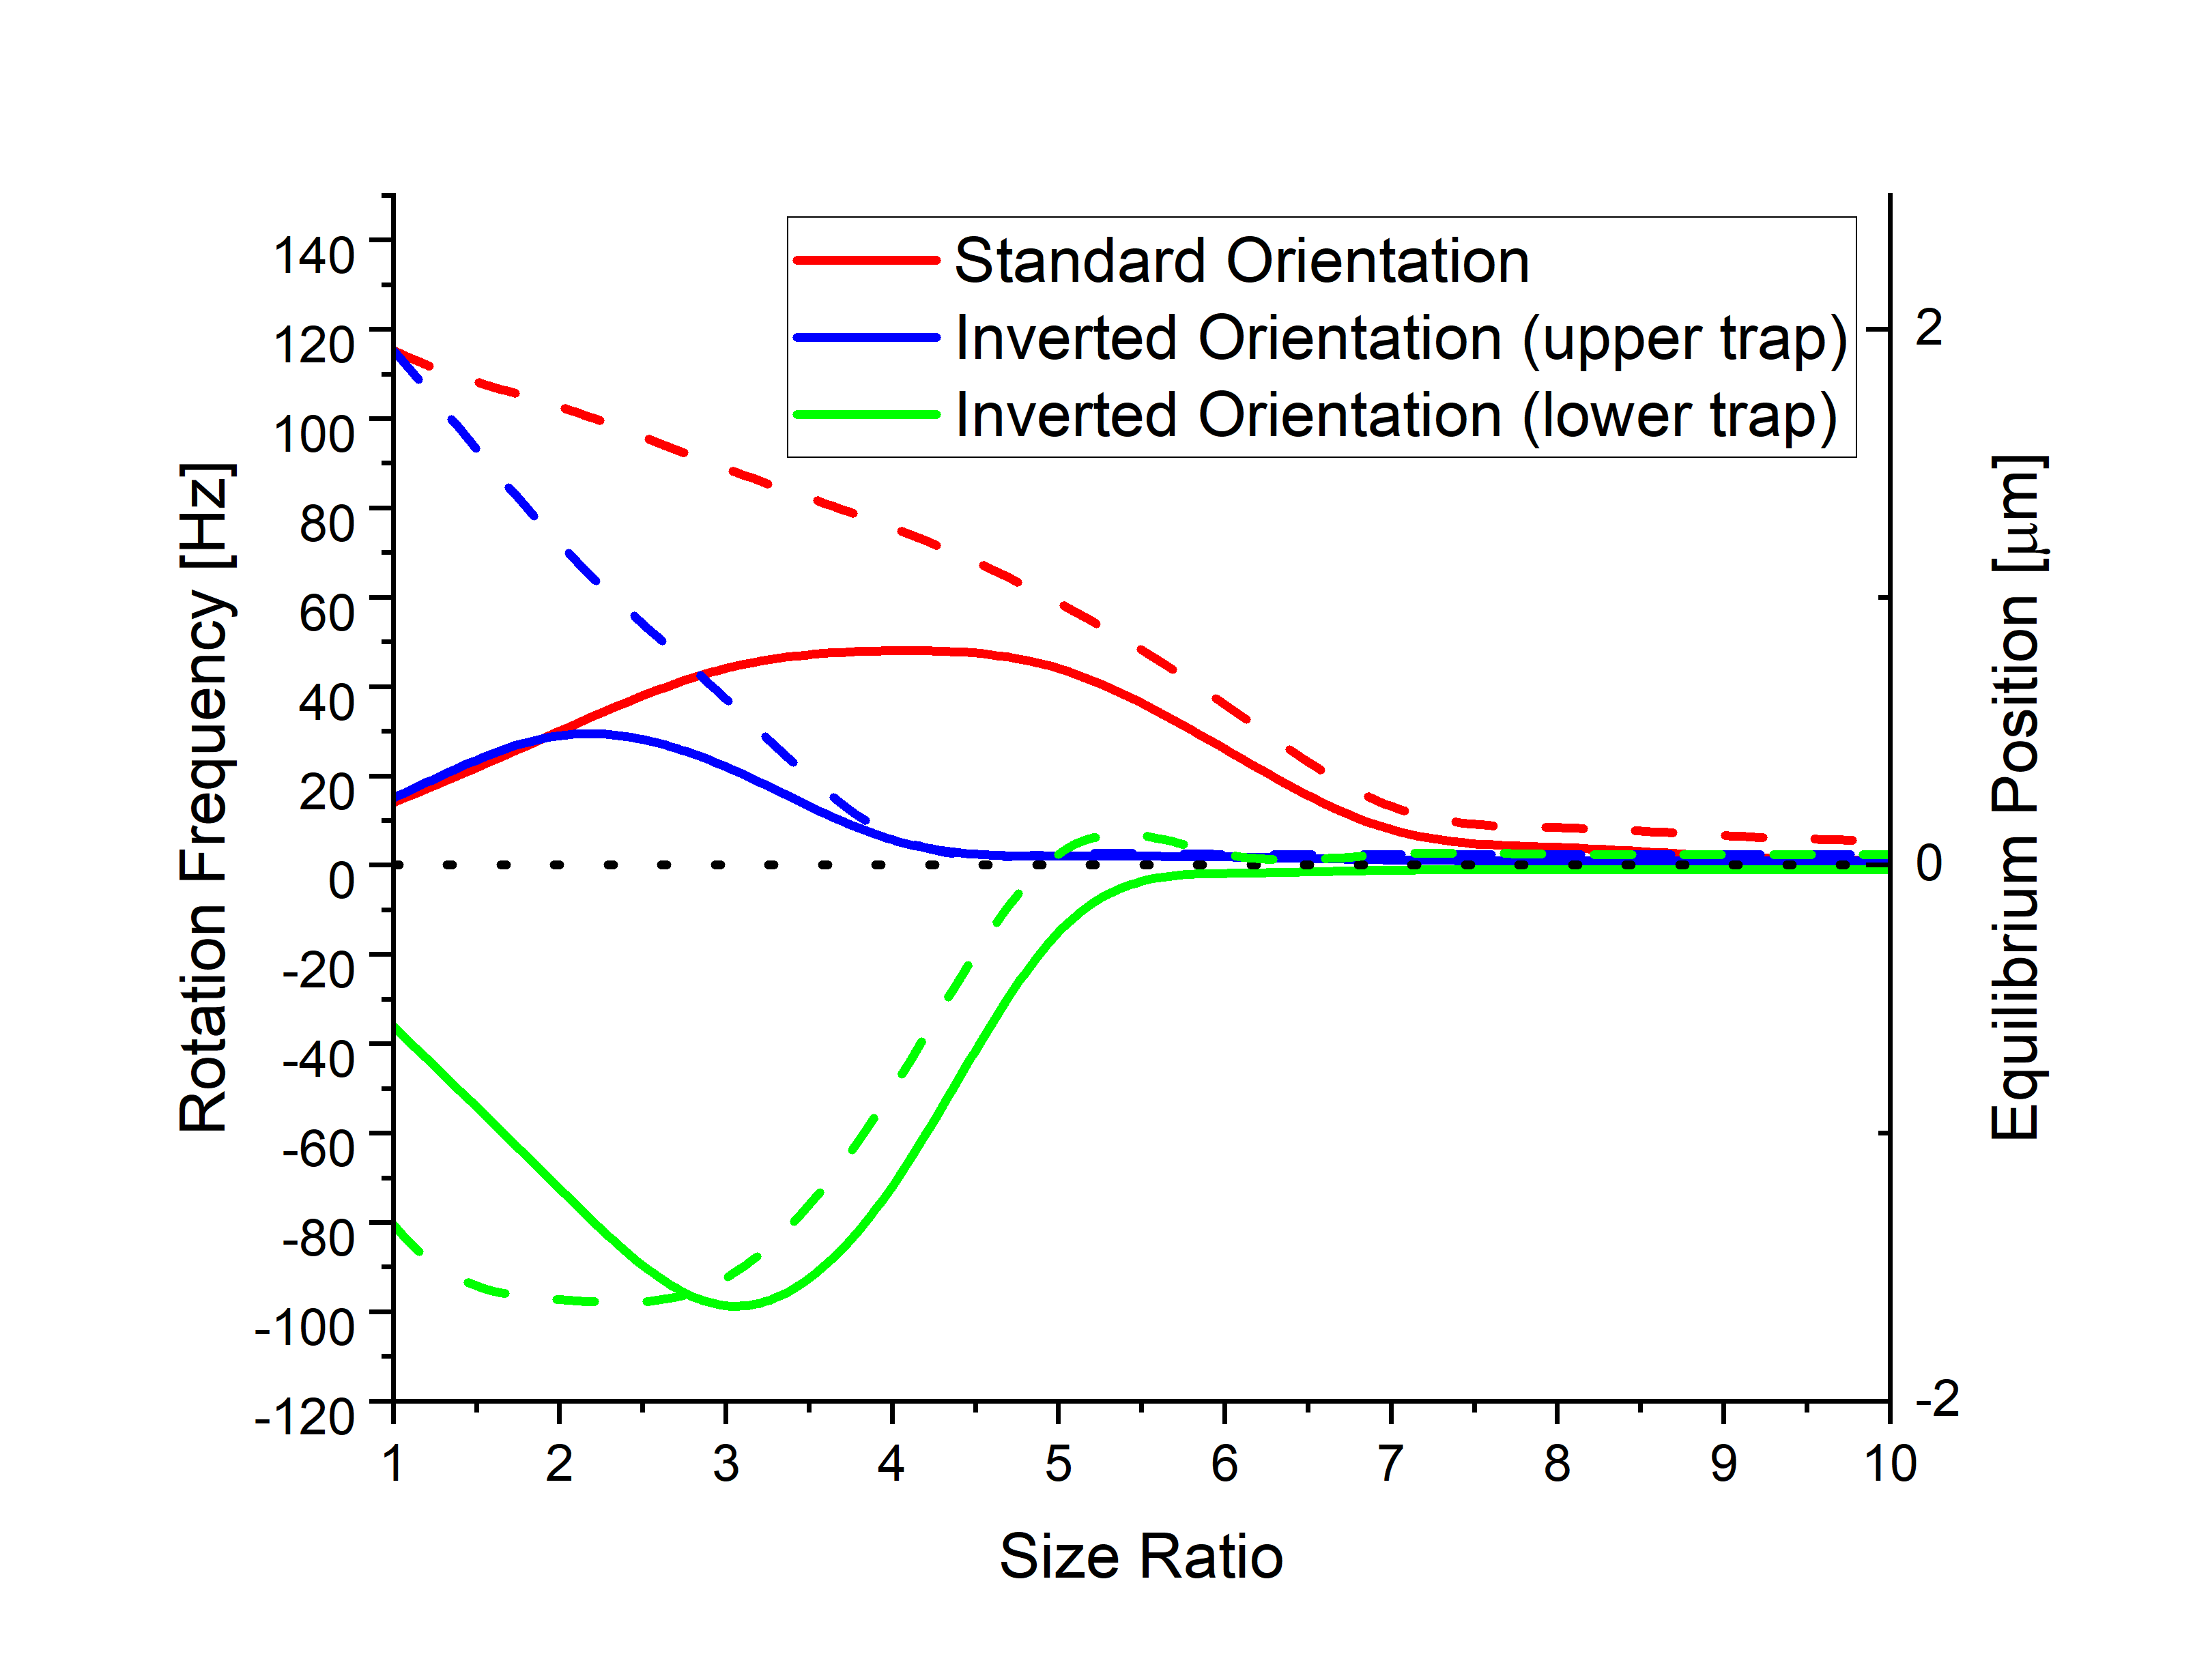
\includegraphics[width=\linewidth]{rotation_rate_vs_size.png}
  \caption{Rotation rate plotted against dimer size ratio while trapped in a
  	circularly polarised beam; a positive rotation rate indicates clockwise 
  	rotation, whereas a negative rotation rate indicates counter-clockwise 
  	rotation. The red line is for the case of a dimer in its 'standard' 
  	orientation. The blue line is for the case when the dimer is in its 
  	'inverted' orientation while trapped above the focus of the beam. And 
  	lastly the green line is for the case when the dimer is in its 
  	'inverted' orientation, but when it is trapped below the focus of the 
  	beam.}
\end{figure}

It is difficult to see from the graph, but the rotation rate never
truly goes down to zero, reaching a minimum of $2\,{\rm Hz}$, which would
imply that a second sphere of radius $200\,{\rm nm}$ is enough to
induce rotational motion. This brings into question what mechanism is
generating the optical torque. We used \textit{mstm} to look at the stokes
parameters from the scattered field from a simple plane wave incident
on a symmetric dimer, the proportion of circularly polarised light is 
minimal compared to the proportion of plane polarised light, which 
indicates that this rotational motion is not due to any inhomogeneity 
in the dimer that might impart angular momentum to the scattered beam - 
as compared to a anisotropic scatterer like vaterite. Therefore the 
rotational motion must be due to 

These results are somewhat contradictory to other work with silica dimers
\cite{Ahn2018, Debuysschere2023,Reimann2018}; previous experiments
have trapped the dimer in an orientation perpendicular to the beam
propagation direction. The rotational motion is attributed to the
dimers asymmetric geometry creating an unbalanced polarisation susceptibility
along its long axis as compared to its short axis; therefore its long
axis is aligned with the polarisation vector and can rotate
freely \cite{Ahn2018}. This however cannot be the case with our
simulations as the dimer rotates about its long axis, meaning there
cannot be an asymmetric axis to align with the beam's polarisation
vector. Furthermore, we see a non-linear increase in the rotational
speed of our dimers with size, the drag torque from the surrounding
fluid is $\propto r^3$ so the expectation is that the rotation
frequency should fall off with increasing size.  This indicates that
the rotational motion is due to the shape asymmetry of the dimer and
not solely due to the beam's angular momentum.  Measurement of this
photo-kinetic force is difficult to achieve due to the fact that
previous analysis was conducted in the Rayleigh regime, where the
polarizability of our dimer can be approximated as:
\begin{align}
  \bold{p}({\bf r},t)
  =
  \alpha_x E_x({\bf r},t)\hat{\bf e}_x
  + \alpha_yE_y({\bf r},t)\hat{\bf e}_y
  + \alpha_zE_z({\bf r},t)\hat{\bf e}_z
\end{align}

where the polarizability is given as a 3D vector for the three
principle Cartesian directions. In order to measure the magnitude of
second order contributions we would need to construct a dipole array
that fully captures the scattering of a dimer. Measuring the optical torque 
makes it clear that the polarizability is a contributing factor to this optical 
rotation phenomena. Rotating a symmetric dimer in the $x-z$ plane reveals 
that while the dimer can be rotated in an orientation perpendicular 
to the beam rotational torque is maximised when rotated while aligned with 
the optical axis.
\begin{SCfigure}
	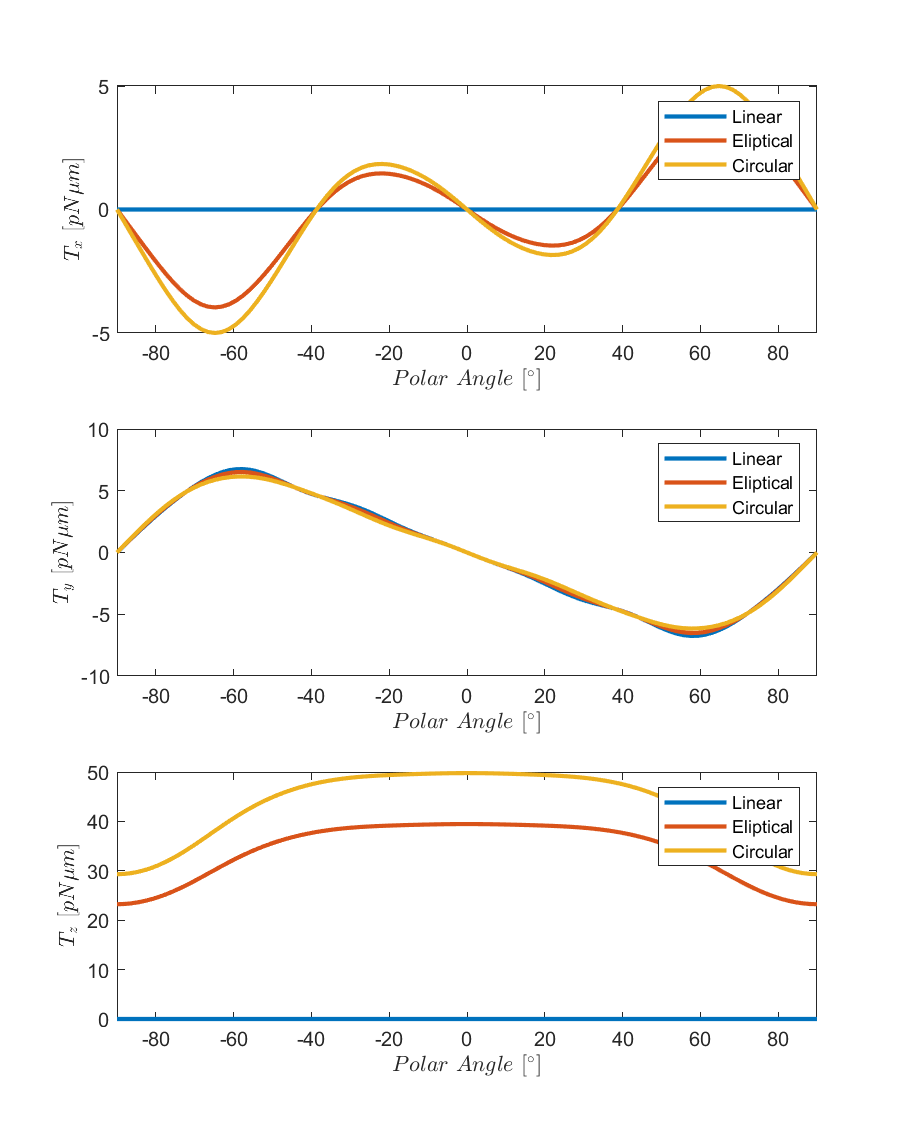
\includegraphics[width=0.65\linewidth,height= 15cm]{torque_different_polarisations.png}
	\caption{Optical torque against polar angle $\theta$ about the three primary axis (top: torque about the x-axis; middle: torque about the y-axis; bottom: torque about the z-axis) on a symmetric dimer in linear, elliptical, and circular polarisation beams. Diagram to the right is for visual clarity about the direction of $\theta$.\vspace{4.5cm}}
\end{SCfigure}
\newpage

\subsection{Gyroscopic Precession using asymmetric dimers}
As mentioned in section~\ref{sec:off-axis} for specificity 
sized dimers there is the potential for non-vertical trapping 
orientations in which the dimer is located in a harmonic 
trap. When trapped by a circularly polarised light these 
dimers exhibit gyroscopic precession. As shown in fig~\ref{fig:gyro} 
the dimer's is rotating about it's long axis (as seen by 
the periodic behaviour of $U_x$ and $U_y$), while also precessing 
around the optical axis of the beam, resulting in a second 
order oscillation in $s_z$.
\begin{figure}[h]
	\centering
	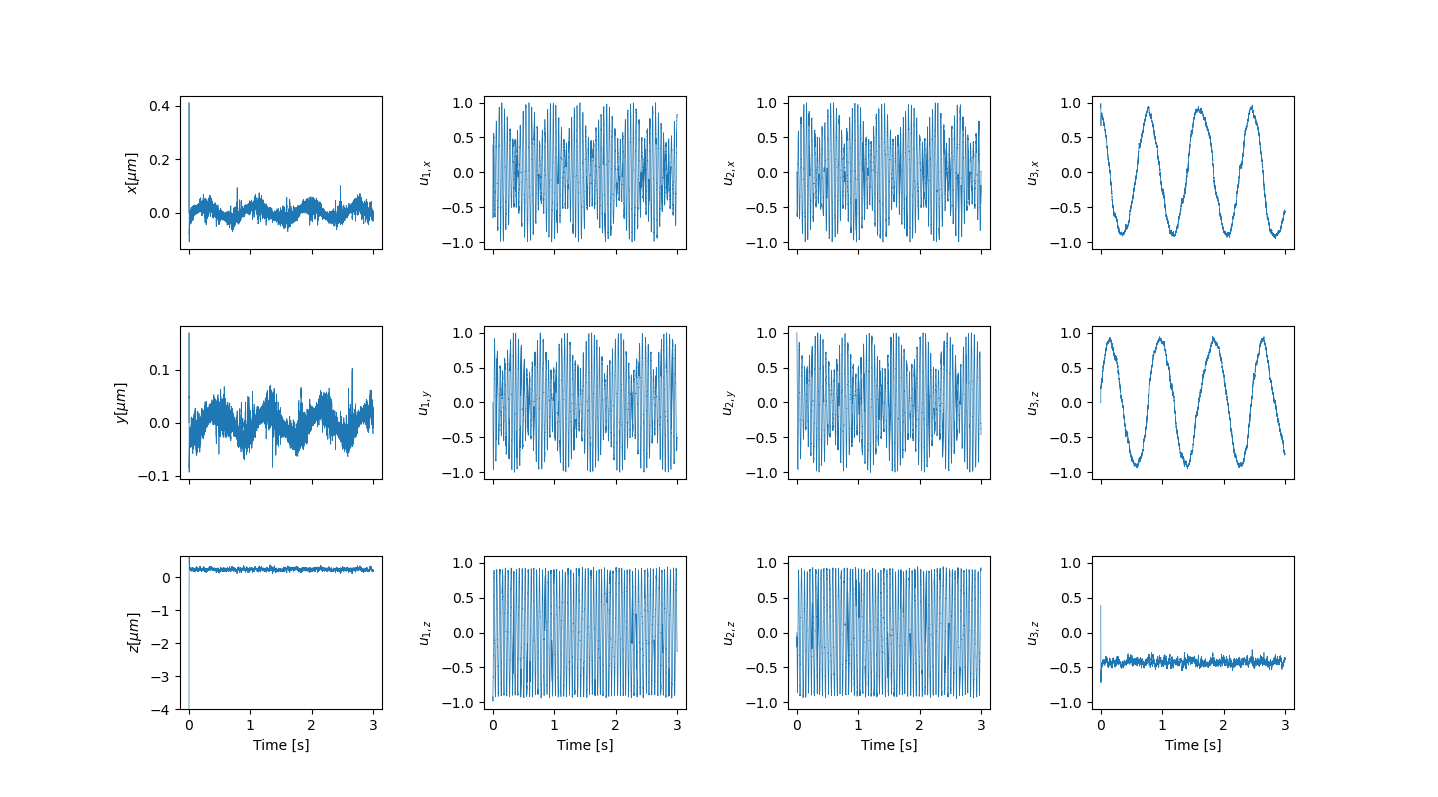
\includegraphics[width=\linewidth]{gyroscopic_precession.png}
	\caption{3 second trajectory of a dimer ($a_{I}/a_{II}=2$) trapped in an 
		off axis orientation with a circular polarised beam ($P= 100\ mW$). 
		The far left column depicts the dimer's centre of mass position with 
		time; middle two columns are the $x$, $y$, and $z$ components of the 
		vectors $u_x$ and $u_y$; last column depicts the components of the 
		vector $u_z$ which defines the dimer's orientation.}
	\label{fig:gyro}
\end{figure}

Applying a Fourier analysis to the above trajectory reveals the 3 fundamental
frequencies typically associated with precession; the $u_{z,1}$ and $x(t)$ 
series show a precession frequency of $~1.33\ Hz$ whereas the series $u_{x,1}$ 
and $u_{y,1}$ show a combined periodic signal - a rotational frequency of 
$~23\ Hz$ and a nutation frequency of $~20\ Hz$. Previous studies into 
amorphous silica nanoparticles found a linear relationship with the 
rotational frequency and the laser power, but no such relationship existed 
with the precession frequency. Our own results shows a similar linear 
relationship with vertically aligned dimers.
\begin{figure}
	\includegraphics[width=\linewidth]{RotationvsPower.png}
	\caption{Rotational frequency vs laser power for a dimer in both vertical orientations.}
\end{figure}

The linear relationship could partly be due to fact that we do not
account for the change in viscous forces with increasing laser power. 
Due to the localised heating effect 
It is far more likely that the rotational frequency reaches a maximum 
value assuming that the bulk fluid can readily absorb the laser.

This gyroscopic motion has been demonstrated previously in nanoparticles 
\cite{Zhu2021, Rashid2018, Hoang2016, Kuhn2016} but has not been observed 
for micron scale aggregates. Since the torque applied to the dimer is 
computed by evaluating the beam coefficients of the scattered field it is 
difficult to apply this result to micro-rheology experiments as one would 
need to know the exact magnitude of the optical torque ahead of time in 
order to make estimations about the local fluid viscosity. This is trivial 
for a birefringent spherical particle, less so for spherical aggregates 
whose equilibrium position and orientation are unknown. However, further 
analysis of the mechanism behind the precessive motion of off-axis dimers
may provide insights into controlling Brownian motion. An experimental work
trying to 'cool' nano-dimers by controlling the motion in all 6 degrees of 
freedom found that even while the rotation about the short axis' could be 
controlled the free rotation around the dimers' long axis resulted in an 
unpredictable torsional vibration \cite{Bang2020}. Understanding how 
rotational motion arises in the Mie-Regieme could allow researchers to 
build a robust theoretical framework to construct beam structures that 
eliminate any unwanted rotational motion from a target particle. Conversely, 
the same framework could allow for precise measurements of the optical 
torque applied to a target particle, allowing for characterisation of 
complex shaped particles' interactions with an optical trap. 

\section{Characterisation of asymmetric dimers via PSD analysis}
As discussed in \ref{sec:simulated_QPD}, one of the methods developed to 
work in conjunction with \cite{Vigilante2020} is a simulated quadrant photo 
diode for as a position detection system. While it is possible to extract 
all of the relevant dynamical information from a simulation, confirming 
the same behaviour in an experimental setting can be challenging if dealing
with a non-birefringent particle.  

As a benchmark we start by considering a single sphere within an optical trap. 
A single silica sphere suspended in water ($a=1\mu m$, $n_p=1.59$, $n_m=1.33$)
is trapped by a focus Gaussian beam and its trajectory was recorded. A 3 second 
is trajectory is a typical measurement time for collecting a power spectrum, 
the spectra was fitted to eq.~\ref{eq:alaised_lorentzian}.
\begin{figure}[h]
	\centering
	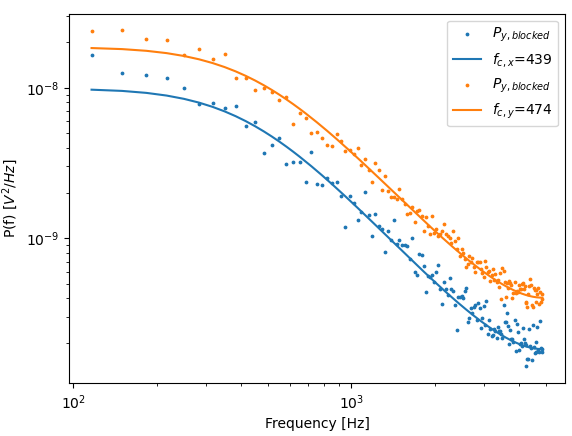
\includegraphics[width=\linewidth]{PSD_sphere.png}
	\caption{Recorded power spectra fitted to eq.~\ref{eq:alaised_lorentzian},
		 scattered points represents the blocked data ($n_b=100$). Corner 
		 frequency for the Lorentzian curves are reported in the legend.}
	\label{fig:psd_sphere}
\end{figure} 

As shown in fig.~\ref{fig:psd_sphere}, the two power spectra report 
different corner frequencies which would be indicate that the trap 
is not perfectly circular. Using \textit{ott} we can compare the 
expected trap strength to what is reported by a quadrant photo diode:

\begin{center}
	\begin{tabular}{ |c|c|c|c|c|c|c| } 
		\hline
		Fitting parameter & \multicolumn{2}{|c|}{\textit{ott} estimates} & \multicolumn{2}{|c|}{QPD fitting} & \multicolumn{2}{|c|}{Simulation fitting}\\
		\hline
		$f_c\ [Hz]$ & 447 & 450 & \parbox{1cm}{\centering 439} & 474 
		& \parbox{1.25cm}{\centering 523} & 513 \\
		$\kappa\ [pN/\mu m]$ & 53.05 & 53.40 & 51.96 & 56.09 & 61.94 & 60.7 \\
		\hline
		Ellipticity &
		\multicolumn{2}{|c|}{8.16 \%} &
		\multicolumn{2}{|c|}{27.17 \%} &
		\multicolumn{2}{|c|}{13.8 \%} \\
		\hline
	\end{tabular}
\end{center}

Where the ellipticity of the beam is given by $e = (1-\kappa_y/
\kappa_x)^{0.5}$ and is a measure of the symmetry of the beam 
wavefront. Its clear from these initial results that the QPD 
is more sensitive to changes along the y-axis than the x-axis 
when compared to the direct \textit{ott} calculations. Typically, 
even an industrial Gaussian beam will produce an elliptical 
diffraction limit spot when heavily focused; in their tutorial 
for optimizing the PSD analysis, Berg and Sorensen reported a 
ellipticity of around 15 \% after a total calibration time of 
81 seconds \cite{BergSoerensen2004}. The reason for this 
discrepancy can be explained partly by the fact that our 
estimation of the trap geometry via \textit{ott} is based on 
the force-displacement curve while the sphere is moving in only 
one direction, whereas the QPD is estimating the trap geometry 
by extrapolating from far field scattering signals. We now 
consider a symmetric dimer in identical simulative conditions.

\begin{center}
	\begin{tabular}{ |c|c|c|c|c|c|c| } 
		\hline
		Fitting parameter & \multicolumn{2}{|c|}{\textit{ott} estimate} & \multicolumn{2}{|c|}{QPD fitting} & \multicolumn{2}{|c|}{Simulation fitting} \\
		\hline
		$f_c\ [Hz]$ & 409 & 334 & \parbox{1cm}{\centering 431} & 424 
		& \parbox{1.25cm}{\centering 274} & 285 \\
		$\kappa\ [pN/\mu m]$ & 48.51 & 39.58 & 51.13 & 50.26 & 32.45 & 33.75 \\
		\hline
		Ellipticity &
		\multicolumn{2}{|c|}{42.8 \%} &
		\multicolumn{2}{|c|}{12.7 \%} & 
		\multicolumn{2}{|c|}{13.8 \%} \\
		\hline
	\end{tabular}
\end{center}

Now we see that the \textit{ott} predicts a more elliptical 
trap compared to the QPD model which says the trap is far
more symmetrical while trapping a symmetric dimer. A potential 
reason that \textit{ott} no longer expects a circular trap 
could be due to how it computes the beam shape coefficients; 
by point matching in the far field before the focus means a 
loss in accuracy for objects that trap above the focus. 
The change in the QPD estimation can be partially explained 
by the fact that rotational effects are not accounted for in 
the Lorentzian power spectra, only translational motion. 
Typically, rotational motion is only ever detected when it 
is periodic (take for example Fig.~\ref{fig:vaterite}), when 
the motion is stochastic the entire power spectra is effected 
making it near impossible to separate the translational and 
rotational contributions from a single power spectra. 

%%%%%%%%%%%%%%%%%%%%%%%%%%%%%%%%%%%%%%%%%%%%%%%%%%%%%%%%%%%%%%%%%%%%%%%%%%%%%%%%
%%%%%%%%%%%%%%%%%%%%%%%%%%%%%%%%%%%%%%%%%%%%%%%%%%%%%%%%%%%%%%%%%%%%%%%%%%%%%%%%
\section{Conclusions}
Considering the simplicity of a scatterer such as a dimer,
one would assume that the dynamics of such an object would be
relatively easy to predict. Simulations of dimers in the Mie regime
show that not only do they have multiple positions and orientations 
in which they can be trapped but also that their interaction
with circularly polarised light is heavily dependent on the axial 
position and trapping orientation. Dimer's have the potential to be used
as adaptive micro-rotors, being simple to synthesise and can be made 
out of any material of choice, but in order for these particles to be
used as such one needs a means of characterising the optical torque
applied. While estimations can be made in the Rayleigh regime due to 
the dimer being treated as point dipole, Mie regime micro rotors require 
an in-depth theoretical description of the mechanism that is creating 
this optical torque. 
